\documentclass[a4paper, 12pt]{article}

\usepackage[dvipsnames]{xcolor} % Code highlighting color
\usepackage[catalan]{babel} % Language 
\usepackage{fontspec} 
\usepackage{fullpage}
\usepackage[a4paper, margin=2cm]{geometry} % To change the margins
\usepackage{graphicx} % Insert images
\usepackage[hidelinks]{hyperref} % Links color
\usepackage[final]{pdfpages}
\usepackage{ragged2e}
\usepackage{wrapfig} %To Text wrap
\usepackage{listings} % Add code
\usepackage{verbatim}
\usepackage{tikz}
\usepackage{subcaption}
\usepackage{multirow}
\usepackage{colortbl}


\usetikzlibrary{arrows, positioning, shapes}

\tikzstyle{vec1} = [rectangle, centered, draw, minimum height = .8cm, minimum width=2.2cm]
\tikzstyle{vec2} = [vec1, minimum width=1.8cm]
\tikzstyle{arrow} = [thick,->,>=stealth]
\tikzstyle{scat} = [ scale=0.8, every node/.style={scale=0.8} ]

\renewcommand*\contentsname{Índex}
\setlength\parindent{0pt}

\lstset{ %
	backgroundcolor=\color{white},   % choose the background color; you must add \usepackage{color} or \usepackage{xcolor}
	basicstyle=\footnotesize,        % the size of the fonts that are used for the code
	captionpos=b,                    % sets the caption-position to bottom
	extendedchars=true,              % lets you use non-ASCII characters; for 8-bits encodings only, does not work with UTF-8
	keepspaces=true,                 % keeps spaces in text, useful for keeping indentation of code (possibly needs columns=flexible)
	keywordstyle=\color{blue},       % keyword style
	numbers=none,                    % where to put the line-numbers; possible values are (none, left, right)
	rulecolor=\color{black},         % if not set, the frame-color may be changed on line-breaks within not-black text (e.g. comments (green here))
	showspaces=false,                % show spaces everywhere adding particular underscores; it overrides 'showstringspaces'
	showstringspaces=false,          % underline spaces within strings only
	showtabs=false,                  % show tabs within strings adding particular underscores
	tabsize=2,	                   % sets default tabsize to 2 spaces
}

\begin{document}
\title{\textsc{Cerca local}}
\author{Marc Asenjo i Ponce de León \and
	Joan Marcè i Igual \and
	Iñigo Moreno i Caireta}
\date{\today}
\maketitle

\section{Implementació estat}
La nostra implementació d'estat utilitza dos vectors de 2 dimensions. Un conté els fitxers que ha demanat cada usuari i l'altre vector, el servidor que serveix aquest fitxer. Així doncs al modificar l'estat només es modifica el segon vector permetent que el primer sigui una variable \verb|static|.

\begin{figure}[ht]
\centering
\begin{minipage}[t]{0.49\textwidth}
\begin{tikzpicture}[auto, align=center, node distance = 0cm, scat]

\node(U1)[vec1] {Usuari 1};
\node(U2)[vec1, right = of U1] {Usuari 2};
\node(U3)[vec1, right = of U2, minimum width = 3cm] { ... };
\node(U4)[vec1, right = of U3] {Usuari n};

\node(F1)[vec2, below = of U1, yshift=-1cm]{Arxiu 1};
\node(F2)[vec2, below = of F1]{Arxiu 2};
\node(F3)[vec2, below = of F2]{...};
\node(F4)[vec2, below = of F3]{Arxiu n};

\node(F5)[vec2, below = of U2, yshift=-1cm]{Arxiu 1};
\node(F6)[vec2, below = of F5]{Arxiu 3};
\node(F7)[vec2, below = of F6]{Arxiu m};

\draw [arrow] (U1) -- (F1);
\draw [arrow] (U2) -- (F5);

\end{tikzpicture}
\caption{Representació del vector de fitxers so\l.licitats per cada petició}
\end{minipage}
\hfill
\begin{minipage}[t]{0.49\textwidth}
\begin{tikzpicture}[auto, align=center, node distance = 0cm, scat]

\node(U1)[vec1] {Usuari 1};
\node(U2)[vec1, right = of U1] {Usuari 2};
\node(U3)[vec1, right = of U2, minimum width = 3cm] { ... };
\node(U4)[vec1, right = of U3] {Usuari n};

\node(F1)[vec2, below = of U1, yshift=-1cm]{Serv 7};
\node(F2)[vec2, below = of F1]{Serv 4};
\node(F3)[vec2, below = of F2]{...};
\node(F4)[vec2, below = of F3]{Serv n};

\node(F5)[vec2, below = of U2, yshift=-1cm]{Serv 2};
\node(F6)[vec2, below = of F5]{Serv 3};
\node(F7)[vec2, below = of F6]{Serv m};

\draw [arrow] (U1) -- (F1);
\draw [arrow] (U2) -- (F5);

\end{tikzpicture}
\caption{Representació del vector dels servidors assignats a cada petició}
\end{minipage}
\end{figure}

\section{Operadors}

S'han  creat dos operadors diferents, tots dos basats en el mateix principi. El primer operador (1)
canvia el servidor que serveix una petició. Donats un identificador
de usuari (\verb|uid|), una petició (\verb|rid|) i un servidor (\verb|sid|). Assigna el servidor \verb|sid|
perquè envii la petició \verb|rid|.

\begin{lstlisting}[language=java ]
public void swapServer(int uid, int rid, int sid);
\end{lstlisting}

El segon operador (2) és igual que el primer però aplicant-ho dos cops de manera que es canvien els servidors 
assignats a dues peticions. Això permet generar successors molt diferents els uns dels altres de manera que
(en teoria) es poden trobar més solucions tot i que el temps d'execució és més elevat.

\section{Estratègies solució inicial}
S'han plantejat dues estratègies generadores de la solució inicial, la primera, per cada petició, assigna
un servidor aleatori que contingui el fitxer demanat; la segona, assigna a cada petició el servidor amb menys
temps de transmissió per aquesta petició. 


\section{Funcions heurístiques}
Tal i com s'explica a l'enunciat s'han de crear dos heurístics, un per tal de minimitzar el temps del servidor
que necessita més temps per transmetre les seves peticions i un altre per minimitzar el temps total de transmissió 
però amb un temps per servidor el més similar possible entre tots els servidors.

Pel primer heurístic s'ha agafat com a valor de l'heurístic el valor de temps del servidor que triga més.

Pel segon heurístic s'ha agafat com a valor de l'heurístic la següent fórmula sobre el conjunt de dades dels temps
de transmissió de cada servidor.
$$\mu\cdot\overline{x}^2 + \sigma^2$$
On $\sigma$ és la variància, $\overline{x}$ és la mitjana i $\mu$ és un factor que s'ha d'escollir experimentalment.

\section{Experiments}
\subsection{}
Es demana escollir el conjunt d'operadors que dóna millors resultats per a la funció heurística que optimitzi el 
primer criteri. Per obtenir els resultats s'han utilitzat 10 llavors diferents, han estat les mateixes 10 tant per l'operador 1 
com pel 2. Als resultats es pot veure que les solucions dels operadors 1 i 2 són molt semblants, la solució
obtinguda amb l'operador 2 és millor però en canvi el temps per trobar la solució és tant gran que ni tan sols s'aprecia
al gràfic pel que s'acaba escollint l'operador 1.

\begin{figure}[h]
\centering
\begin{minipage}[t]{0.48\textwidth}
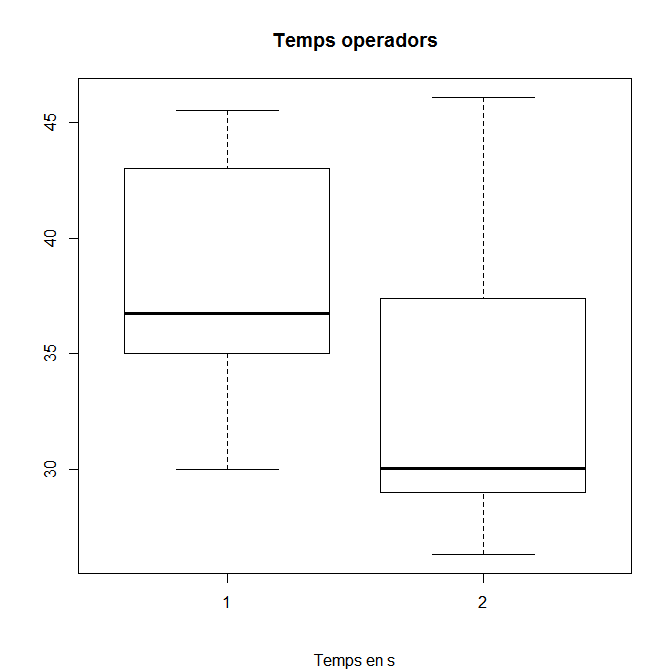
\includegraphics[width=\linewidth]{operadors}
\caption{Box plot dels temps màxims dels resultats al utilitzar l'operador 1 i 2}
\end{minipage}
\hfill
\begin{minipage}[t]{0.48\textwidth}
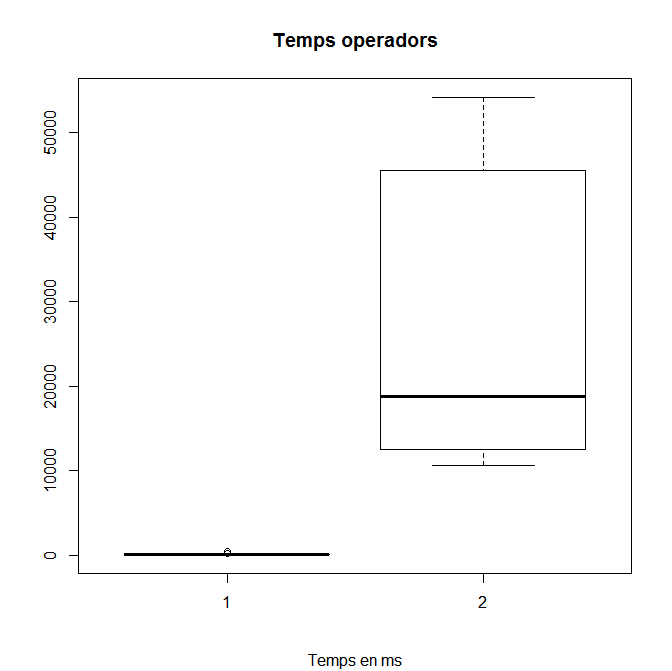
\includegraphics[width=\linewidth]{operadorsT}
\caption{Box plot dels temps que es triga en calcular la solució amb els operadors 1 i 2}
\end{minipage}
\end{figure}

\begin{table}[h!]
\begin{tabular}{l | l || l | l}
	\multicolumn{2}{c||}{Operador 1} & \multicolumn{2}{|c}{Operador 2} \\
	\hline
	Resultat (s) & Temps (ms) & Resultat (s) & Temps (ms) \\
	\hline
	35 & 415 & 30 & 45.523 \\
	41 & 110 & 29 & 54.225 \\
	35 & 168 & 37,4 & 16.391 \\
	35,5 & 104 & 34 & 11.272 \\
	45,5 & 81	& 46,1 & 10.543 \\
	35,5 & 91 & 30,1 & 15.442 \\
	43 & 33 & 28,4 & 34.781 \\
	30 & 89 & 29,9 & 21.260 \\
	38 & 53 & 40,3 & 12.497 \\
	44 & 79 & 26,3 & 47.050 \\
\end{tabular}
\caption{Resultats i temps obtinguts amb els operadors 1 i 2}
\end{table}

\newpage
\subsection{}
Es demana comparar l'estratègia de generació de la solució inicial amb els criteris de l'apartat anterior. També s'han utilitzat 10
llavors diferents per obtenir els paràmetres inicials. 

\begin{minipage}{\textwidth}
\centering
\begin{minipage}[b]{0.45\linewidth}
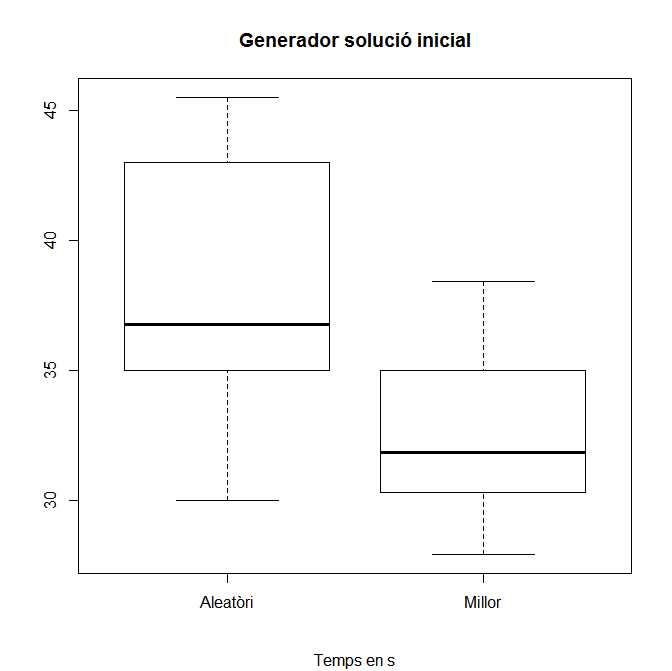
\includegraphics[width=\linewidth]{generador}
\captionof{figure}{Box plot dels temps màxims dels resultats}
\end{minipage}
\hfill
\begin{minipage}[b]{0.45\linewidth}
	\centering
	\begin{tabular}{l || l}
		Aleatori & Millor servidor \\
		\hline
		35 & 32,8 \\
		41 & 35,6 \\
		35 & 32,4 \\
		25,5 & 30,3 \\
		45,5 & 38,4 \\
		35,5 & 29,7 \\
		43 & 35 \\
		30 & 27,9 \\
		38 & 30,6 \\ 
		44 & 31,3 \\
	\end{tabular}
	\captionof{table}{Resultats (en segons) dels dos algoritmes de generació}
\end{minipage}
\end{minipage}

\subsection{}
Es demana determinar els paràmetres del Simmulated Annealing amb el mateix escenari que els experiments
anteriors.

\begin{table}[h!]
\begin{tabular}{l | l | l | l | l|}
	\multicolumn{1}{c}{} & \multicolumn{4}{c}{$\lambda$} \\
	\cline{3-5}
	\multicolumn{2}{c|}{} & 0,001 & 0,01 & 0,1 \\
	\cline{2-5}
	\multirow{3}{*}{$k$}
	& 1 & \cellcolor{Green!50} 25.610 & \cellcolor{Green} 25.497 & \cellcolor{Red!60}30.733 \\
	& 1e2 & \cellcolor{Goldenrod!70}25.867 & \cellcolor{Green!60}25.577 & \cellcolor{Red!60}30.788 \\
	& 1e4 & \cellcolor{Goldenrod}26.666 & \cellcolor{Green!40}25.715 & \cellcolor{Red!60}30.474 \\
	\cline{2-5}
\end{tabular}
\end{table}

\section{Comparació resultats}

\end{document}